\documentclass[a4paper,10pt]{article}
\usepackage[utf8]{inputenc}
\usepackage{graphicx}
\usepackage{geometry}
 \geometry{
 a4paper,
 left=40mm,
 right=30mm,
 top=30mm,
 bottom=30mm,
 }

%opening
\title{}
\author{}
\pagenumbering{gobble}
\begin{document}

\begin{center}
 \LARGE \textbf{Bad Rear View Mirror Rejection System}\\
 \large Ir. Apriani K. MSc, Irwansyah ST. MT, and Achmadi\\
 \large Photonic Engineering Lab, Engineering Physics Dept, Sepuluh November Institute of Technology, Indonesia\\
 \large fotonikits@gmail.com
\end{center}


\begin{abstract}

This work was propose to create an industrial-based system that capable to test a rear view mirror and reject the rear view mirror if it was bad quality.
Rear view mirror analized using computer to get it's reflection distorsion level.
As Indonesian National Standard (SNI) rules, if reflection distorsion level more than 7,then rear view mirror will rejected.
The system only working with 3 subsystem,
 a computer with reflection distorsion level measurement algorithm,
 a robotic arm that can grip rear view mirror and move it between two positions,
 a reflection pattern with webcam that can capture mirror reflected pattern. 
After testing, this system can evaluate reflection distorsion level of Honda's rear view mirrors.
This rear view mirrors collectioan used as standard to test the system.
The result is reflection distorsion level for this rear view mirrors set is between 1,7 and 2,8 which still usable for automotive usage.
The algorithm to get reflection distorsion level run on a computer with Linux 3.13 and Octave 3.8.1.
 
\end{abstract}

\begin{center}
 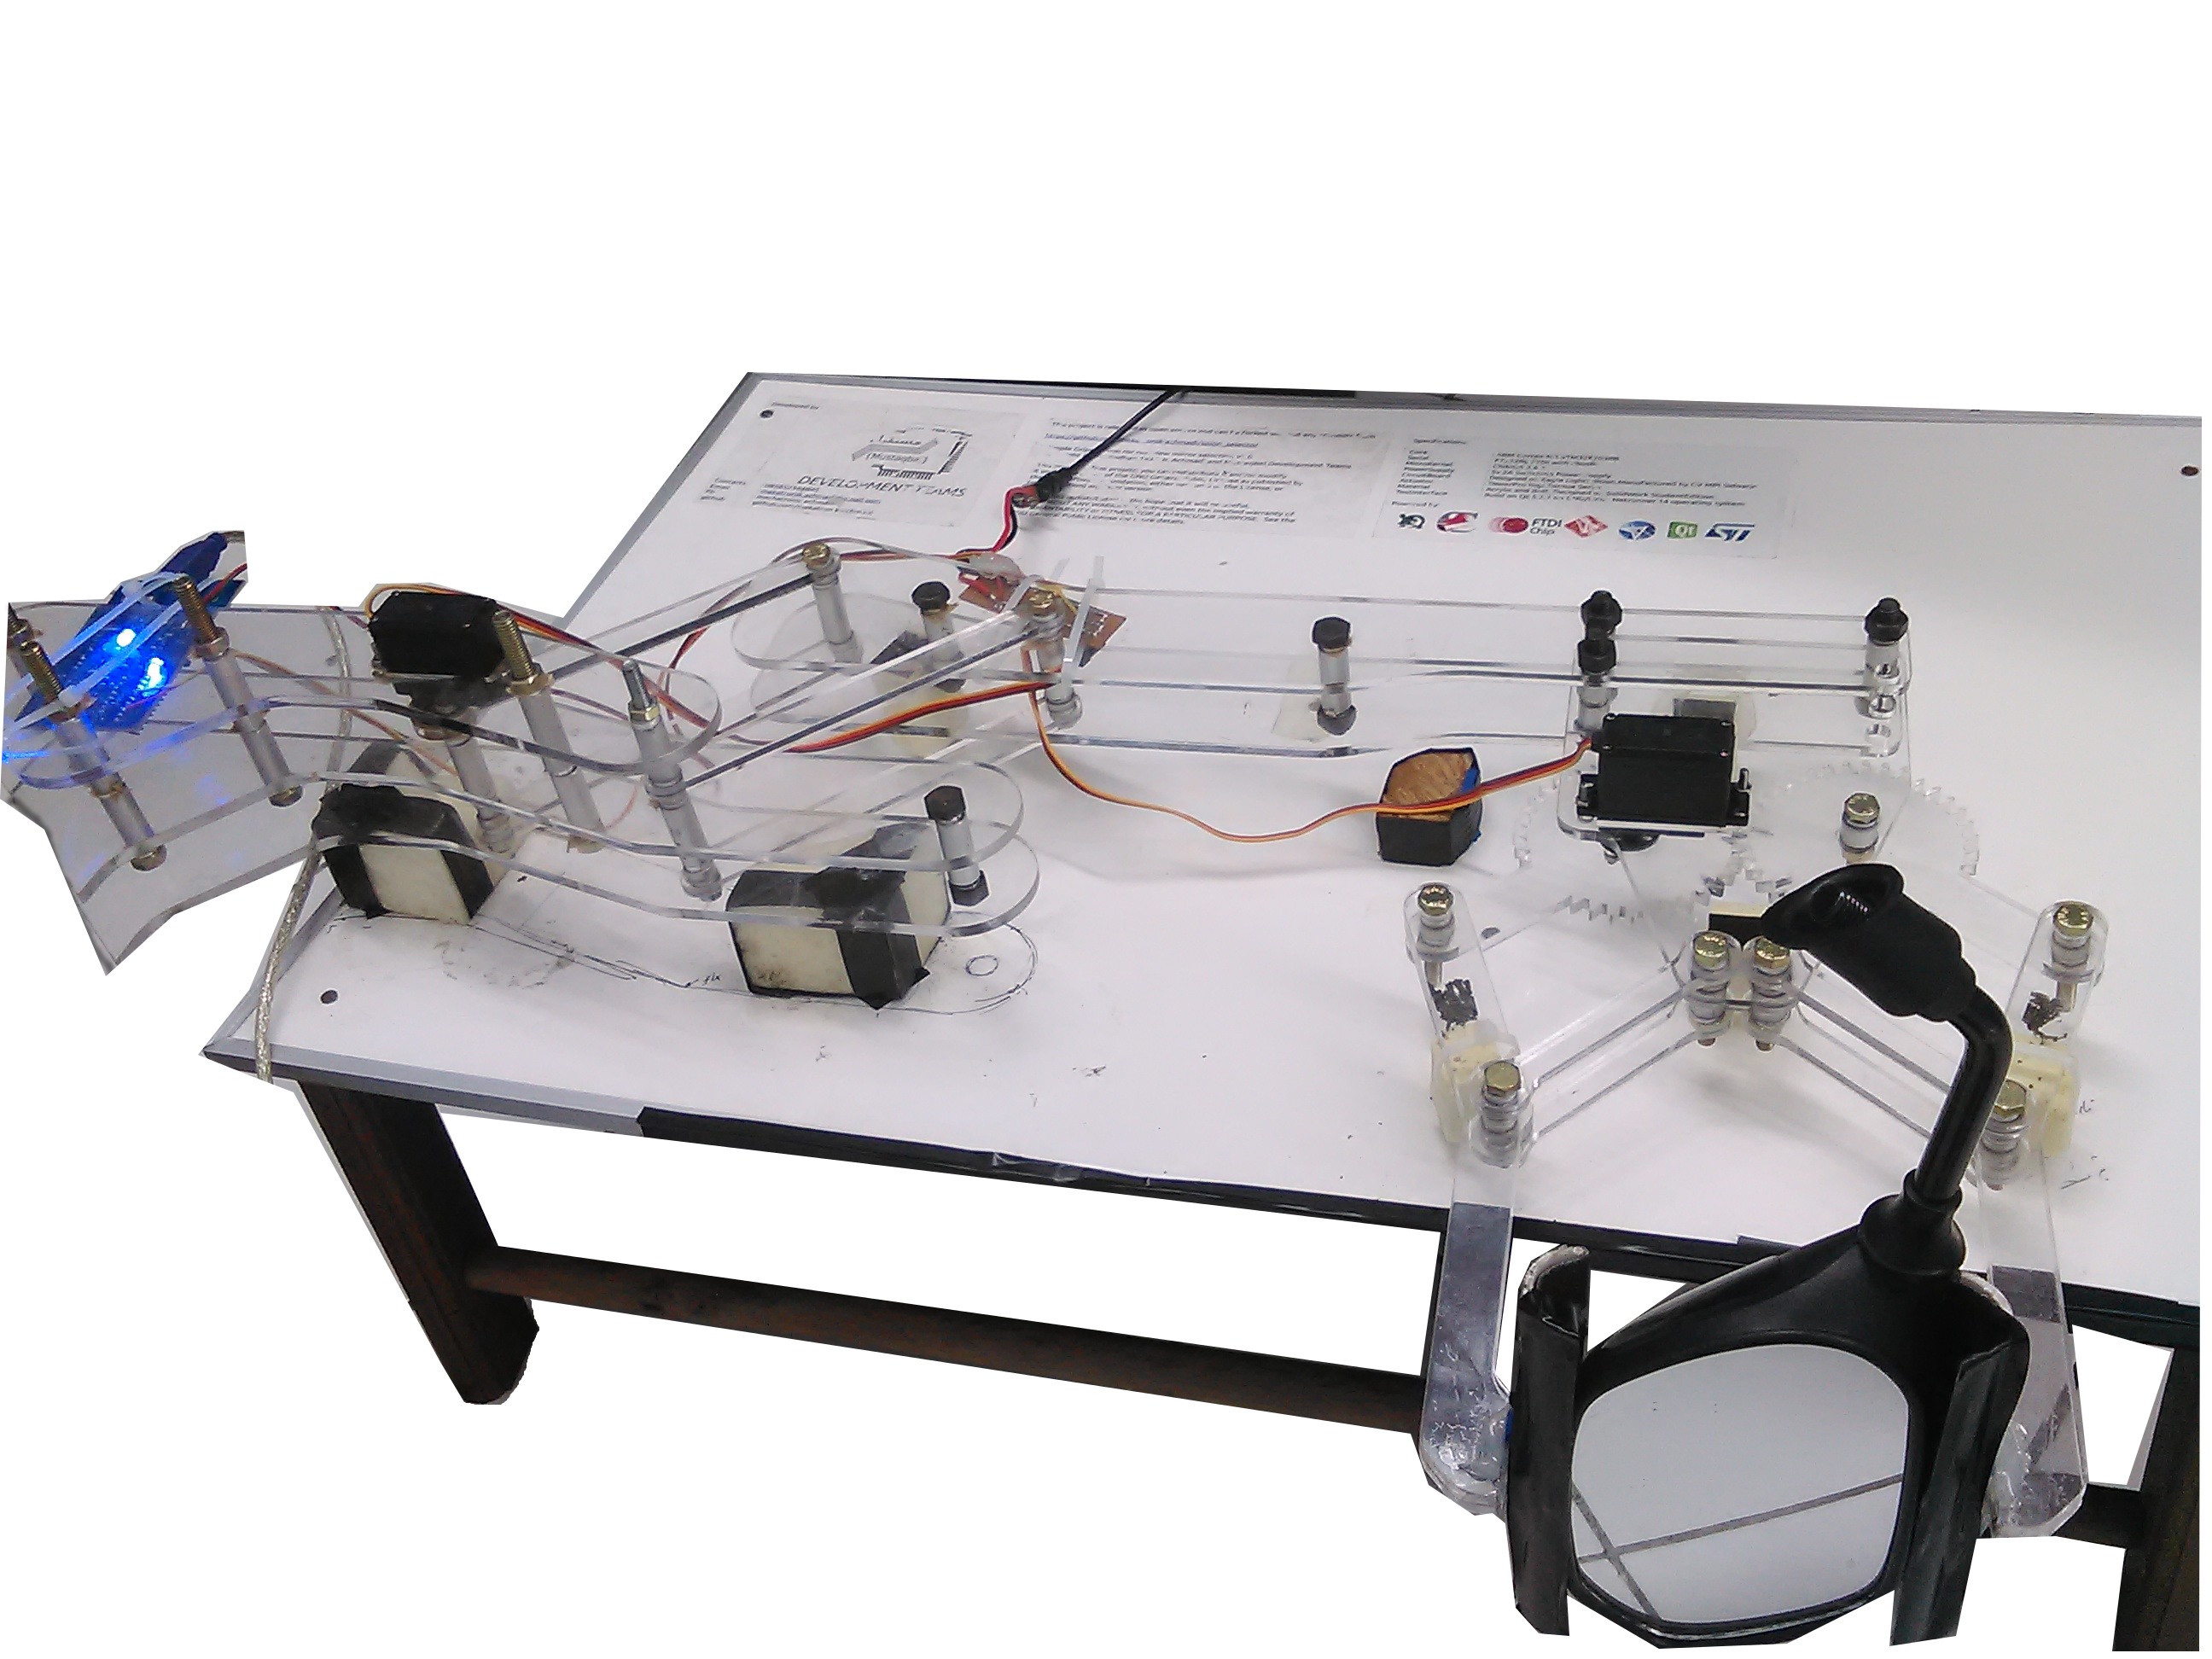
\includegraphics[width=200pt]{selected_system}\\
 \textit{\textbf{Figure1.} Current system design}
\end{center}

\textit{\textbf{Keyword:} reflection distorsion, rear view mirror, rejection system}

\begin{thebibliography}{}
    \bibitem{opencv_intro} OpenCV Team \textit{The OpenCV Reference Manual} 2014
    \bibitem{hsv} Phillips, Dwyne \textit{Image Processing in C} 2000
    \bibitem{improc1} Zhou, Huiyu \textit{Digital Image Processing Part I} 2010
    \bibitem{octave}Eaton, John W \textit{GNU Octave, A high-level interactive language for numerical computations} 1997
    \bibitem{stm32}Brown, Geoffrey \textit{Discovering the STM32 Microcontroller} 2013
    \bibitem{sni}Badan Standard Nasional, \textit{Selective Disemination of SNI Information} 2013
    \bibitem{mirror} Savarese, Silvio \textit{What do reflections tell us about the shape of a mirror?} 2004
\end{thebibliography}

\end{document}
